\documentclass[11pt,a4paper]{article}
\usepackage[utf8]{inputenc}
\usepackage[T1]{fontenc}

\usepackage[dvipsnames,usenames]{color}
\usepackage[colorlinks=true,urlcolor=Blue,citecolor=Green,linkcolor=BrickRed]{hyperref}
\usepackage[usenames,dvipsnames]{xcolor}
\urlstyle{same}

\usepackage{amsthm,amsmath,amssymb,mathabx}
\usepackage{fullpage}
\usepackage[ruled,noend,linesnumbered]{algorithm2e}     
\usepackage{enumerate,comment}
\usepackage{url}
\usepackage[capitalise]{cleveref}
\usepackage{todonotes}
\usepackage{tikz}
\usepackage[noadjust]{cite}
\usepackage{xspace}
\usepackage{graphicx}
\usepackage{float}
\usepackage{amsfonts}
\usepackage{color}
\usepackage{array}

%\pagestyle{plain}

\newcommand{\ceil}[1]{\left\lceil #1 \right\rceil}
\newcommand{\floor}[1]{\left\lfloor #1 \right\rfloor}
\newcommand{\poly}{\text{poly}}

\newcommand{\Oh}{{O}}

% For cleverref compatibility
\newtheorem{theorem}{Theorem}[section]
\newtheorem{algo}{Algorithm}[section]
\newtheorem{corollary}{Corollary}
\newtheorem{lemma}{Lemma}
\newtheorem{observation}{Observation}
\newtheorem{fact}[theorem]{Fact}
\theoremstyle{definition}   
\newtheorem{definition}{Definition}
\usepackage{authblk}
\theoremstyle{remark}
\newtheorem{example}[theorem]{Example}
\newtheorem*{claim}{Claim}
\newtheorem{case}{Case}
\newtheorem{invariant}{Invariant}
\newtheorem{step}{Step}[section]

\newtheorem{property}[theorem]{Property}
\newcolumntype{R}[1]{>{\raggedleft\let\newline\\\arraybackslash\hspace{0pt}}m{#1}}

\begin{document}

\title{Dispersion on Trees\thanks{The research was supported in part by Israel Science Foundation grant 794/13.}}
\author[1]{Pawe\l{} Gawrychowski}
\author[1]{Nadav Krasnopolsky}
\author[2]{Shay Mozes}
\author[1]{Oren Weimann}
\affil[1]{University of Haifa, Israel}
\affil[2]{IDC Herzliya, Israel}


\date{}
\maketitle

\begin{abstract}
In the dispersion problem, we want to select $k$ nodes of a given graph so as to maximize
the minimum distance between any two chosen nodes. This can be seen as a generalization
of the independent set problem, where the goal is to select nodes so that the minimum distance
is larger than 1.
We design an optimal $\Oh(n)$ time algorithm for the dispersion problem on trees consisting
of $n$ nodes, thus improving the previous $\Oh(n\log n)$ time solution. 
We also consider the weighted decision version, where the goal is to find a set of nodes of total weight at least $k$ such that any two nodes are at distance at least $\lambda$. For this problem we present tight $\Theta(n\log n)$ upper and lower bounds. 
%For the optimization version, where we wish to maximize  $\lambda$, we present an $\Oh(n\log^2n)$ upper bound improving the previous $\Oh(n\log^4 n)$ time solution. 
\end{abstract}

\section{Introduction}

\emph{Facility location} is a family of problems dealing with the placement of facilities on a network in order to optimize certain distances between the facilities, or between facilities and other nodes of the network. Facility location problems are usually if not always NP-hard on general graphs. There is a rich literature on approximation algorithms for general graphs (see e.g.\cite{DavidB.Shmoys1997,Vazirani2003} and references therein) as well as exact algorithms for restricted graph families. In particular, many linear and near-linear time algorithms were developed for facility location problems on edge-weighted trees.   


In the most basic problem, called \emph{$k$-center}, we are given an edge-weighted tree with $n$ nodes and wish to designate up to $k$ nodes to be facilities, so as to minimize the maximum distance of a node to its closest facility. This problem was studied in the early 80's by Megiddo et al.~\cite{Megiddo1981} who gave an $\Oh(n\log^2n)$ time algorithm that was subsequently improved to $\Oh(n\log n)$ by Frederickson and Johnson \cite{Frederickson1983}. In the early 90's, an optimal $\Oh(n)$ time solution (also for more general variants such as placing facilities on any point along an edge) was given by Frederickson \cite{Frederickson1991a} using a seminal approach based on parametric search. 
%
A related problem, also suggested in the early 80's  \cite{Becker1982,Perl1981}, is \emph{$k$-partitioning}. In this problem the nodes have weight and we wish to delete $k$ edges in the tree so as to maximize/minimize the weight of the lightest/heaviest resulting subtree. This problem was also solved by Fredrickson in $\Oh(n)$ time \cite{Frederickson1991} and also uses his parametric search. 

\paragraph{The dispersion problem.}
A problem that has yet to be solved in linear time is the {\em $k$-dispersion} problem. In this problem, the goal is to designate $k$ nodes as facilities so as to maximize the distances among the facilities.  In other words, we wish to select $k$ nodes that are as spread-apart as possible. This can be seen as a generalization of the classical maximum independent set problem (that can be solved by binary searching for the largest value of $k$ for which the minimum distance is at least 2).  

  We consider the optimization version of the dispersion problem as well as the decision version (also called the {\em feasibility test} in \cite{Frederickson1991,Bhattacharya1991}).
For a subset of nodes $P$, let $d(u,v)$ denote the distance between nodes $u$ and $v$ and let $f(P)=\min_{u,v\in P} \{d(u,v)\}$.

\begin{itemize} \item {\em The Dispersion Optimization Problem.} Given a tree with non-negative edge lengths, and a  number $k$, find a subset of nodes $P$ of size $k$  such that  $f(P)$ is maximized. 

\item  {\em The Dispersion Decision Problem.}  Given a tree with non-negative edge lengths, a number $k$, and a number $\lambda$, find a subset of nodes  $P$ of size $k$ such that  $f(P)\geq\lambda$. 

\end{itemize}

The fastest algorithms for the above problems were given in the early 90's by Bhattacharya and Houle \cite{Bhattacharya1991}. 
They showed that the decision version can be solved in  $\Oh(n)$ time and that the optimization problem can be solved in $\Oh(n\log n)$ time. 
%, improving on an earlier $\Oh(kn+n\log n)$ solution for single-path trees given by Wang and Kuo~\cite{Wang1988}. 
They also considered the case where nodes have weights and the goal is to select nodes with total weight at least $k$. For the weighted optimization problem, they gave an $\Oh(n\log^4 n)$ time solution. %We present a faster $\Oh(n\log^2 n)$ time algorithm. 



\paragraph{Our result and techniques.}

Building on the framework of Frederickson, we give an $\Oh(n)$ time algorithm for the optimization problem. 
We also consider the weighted decision problem. 
We show show a lower bound of $\Omega(n\log n)$ in the algebraic decision tree model and complement this with a matching $\Oh(n\log n)$ upper bound.
%, which is then used to construct our $\Oh(n\log^2n)$ time solution for the weighted dispersion problem using the standard parametric search paradigm of Fredrickson. 


While our final goal is an optimal linear time algorithm for the dispersion optimization problem, we start
with a slower $O(n\log\log n)$ time solution, which we then improve first to $O(n\log^{*}n)$
and then finally to $O(n)$ by gradually introducing new ideas.

The starting point is a simple linear time solution for the decision problem, presented in Section~\ref{linear F.T.}, 
which is similar to the one presented in \cite{Bhattacharya1991}.
Once we have an efficient feasibility test, we can solve the optimization problem we binary searching for the
answer. However, we do not want the running time to depend on the upper bound on the largest possible
distance between two nodes in the tree.  This can be mitigated by observing that the answer is always
a distance between two nodes and constructing an implicit representation
of all possible $O(n^{2})$ distances and binary searching over this representation. More precisely, the representation
consists of $O(n)$ matrices $M_{i}$, where each $M_{i}$ is row- and column-monotone, the total side length
of all the matrices is $O(n\log n)$, and we can provide constant-time access to any entry after $O(n\log n)$
time preprocessing. Then it is not difficult to see that $O(\log n)$ calls to the feasibility test are enough to
find the answer. This results in an $O(n\log n)$ time algorithm. There are two bottlenecks that make decreasing
the running time challenging: we need to avoid the $O(n\log n)$ preprocessing for capturing all the relevant
distances and also need a \emph{sublinear} feasibility test.

We present a sublinear feasibility test in Section~\ref{sublinear f.t.}. The gist of it is a method for partitioning
the tree into fragments, preprocessing every fragment, and then iterating over the fragments in the query.
The standard method for such partitioning is the micro-macro decomposition, where every fragment is
of size $O(x)$, there are $O(n/x)$ fragments, and each fragments contains at most two boundary nodes
incident to nodes in other fragments. We extend it to guarantee that one boundary node is always the
root of the fragment and call the other boundary node the hole. Then we observe that the linear feasibility test
can be seen as a bottom-up computation on the tree. Now we would like to simulate it by jumping over whole 
fragments: after simulating on the subtree rooted at the hole we would like to extend to the whole
subtree rooted at the root of the fragment in $o(n)$ time. This requires preprocessing the fragments,
in particular we need to narrow down the range of possible answers so that for any two nodes in the same
fragment we know if they can be both included in an optimal solution. We are able to determine this
for \emph{most} of the fragments by plugging in the parametric search method of 
Frederickson\cite{Frederickson1991}. 

Frederickson used his parametric search method to solve several problems on trees, in particular
the max-min tree $k$-partitioning~\cite{Frederickson1991}. This is very similar to dispersion and it might
seem that actually these two problems are equivalent. In fact, they are equivalent in the one-dimensional case,
i.e., on a path. The basic idea of this reduction, is to switch between the edges and vertices, i.e. create a new path, where each of the edges is a node in the original path, and each of the points is an edge originally. We assign the same weights, so now we have weights on the points, and run the $k$-partitioning algorithm.

However, such equivalence seems problematic for general trees. Given that these two problems look similar, it should not be surprising that our solution uses similar
ideas, at least at a high level. However, many details and tricks are actually different, and we believe
that some of our techniques might be somehow simpler than his. %TODO explain more
In particular, our algorithm is based on the (tweaked) micro-macro decomposition and the heavy path
decomposition, which are both very standard data structure tools, instead of the less standard
decompositions used by Frederickson.%TODO explain more?

After the initial preprocessing, for any two nodes in most of the fragments we know if they can be
both included in the solution. This allows us to prepare for every possible result of running the
bottom-up computation in the subtree rooted at the hole so that we are able to jump over the whole
fragment in $O(\log x)$ time. This is done by looking at the path from the hole to the root of the
fragment and running the bottom-up computation for all subtrees hanging off from it. This allows
us to conceptually trim the fragment and think of it as a caterpillar, that is, a path connecting
the hole with the root with some additional leaves attached to its nodes. Such caterpillars have
sufficiently simple structure so that, with some additional simple precomputation, after receving
the results of the bottom-up computation in the subtree rooted at the hole, essentially we need
to binary search over the caterpillar and then return the precomputed answer. By appropriately
setting up $x$ to balance the preprocessing and the query time, we obtain an $O(n\log\log n)$
time algorithm.

The bottleneck in the obtained $O(n\log\log n$) time algorithm is the preprocessing time necessary
to construct a sublinear feasibility test. Therefore, we proceed to construct a sequence of
faster and faster feasibility tests. The first of them is just the vanilla linear time feasibility test.
Then, we iteratively use the current feasibility test to construct the next (faster) feasibility test.
Every iteration uses an appropriately chosen parameter $x$ for the micro-macro decomposition
as to guarantee that the construction time is $O(n)$. The parameters grow exponentially,
so after $O(\log^{*}n)$ iterations we obtain the desired efficient feasibility test, which is then
used as previously.

The main difficulty in obtaining the $O(n)$ time algorithm is that now we cannot afford construct each
micro-macro decomposition separately. However, this can be overcome by making each decomposition
a refinement of the previous one. With some care, all decomposition can be then constructed in
$O(n)$ total time. We believe that this (simple) trick is of independent interest. Then, there
are some additional details in how we preprocess every fragment. We cannot afford to touch
every node of every fragment at every level. Therefore, we take a closer look at how a fragment
decomposes into previous fragments. With some care, the results of preprocessing the previous
fragments can be reused while adding some extra work that amortizes to $O(n)$ over all decompositions.

\section{Linear algorithm for the feasibility test}\label{linear F.T.}
%\begin{algo} \label{unWeightedFeasibilityAlgo}
We show a recursive linear algorithm. At each step of the recursion, we would like to provide a valid solution with maximal cardinality for the current subtree, given some $\lambda$, i.e., the algorithm will maintain the following invariant:
\begin{invariant}\label{Maximality of P and distance of closest node invariant}
For every node of the tree, $r$, the algorithm produces $P$, a subset of the vertices of the subtree rooted at $r$, s.t. $f(P)\geq\lambda$ and $|P|$ is maximal. Out of all such valid subsets with maximal cardinality, the distance between $r$ and the node closest to it is maximized in $P$.
\end{invariant}
In each step we are given a root vertex $r$, its children nodes $r_{1},r_{2},...,r_{k}$, and for each child we are given a maximal valid solution for the feasibility test on its subtree. We would like to produce a maximal valid solution for the feasibility test on $r\text{'s subtree}$.
Denote by $P_{1},...,P_{k}$ the solutions for the feasibility test on each subtree rooted at a child of $r$.
\begin{definition}
For any subtree of $T$ rooted at node $r$, and a valid solution $P$ for a feasibility test on the subtree (i.e. $f(P)\geq\lambda$), we call a node $u\in P$, s.t. $d(r,u)<\frac{\lambda}{2}$, the \emph{candidate} node of the subtree (or a candidate with respect to $r$). We call the vertices in $P$ that are not the candidate (i.e. every node $v \in P$ s.t. $d(r,v)\geq \frac{\lambda}{2}$), \emph{certain} (w.r.t $r$). When it is clear from the context, we will not explicitly mention which subtree we are referring to.
Note that for any vertex $x$, a valid solution to the feasibility test on $T_x$ contains at most one candidate vertex.
\end{definition}

\paragraph{The recursion step} Given $P_{1},...,P_{k}$, we would like to produce a solution for $r$'s subtree.
\begin{enumerate}
\item Put in $P$ all the vertices in $P_{1},...,P_{k}$, except for the candidate vertices.
\item Take all candidate nodes $u$ s.t. $d(u,r) \geq \frac{\lambda}{2}$ (i.e. they are certain w.r.t $r$).
\item If it exists, take $u'$, the candidate node farthest from $r$ s.t. $d(u',r) < \frac{\lambda}{2}$ and $d(u',x)\geq \lambda$, where $x$ is the closest node to $u'$ we have chosen so far.
\item Check if it is possible to take $r$ into the solution by looking at the closest vertex to it we have already put in $P$. If possible, put $r$ in the solution.
\end{enumerate}
Iterating over the input tree bottom-up as described, will provide us with the solution to the Dispersion decision problem as the output for the root of the tree.

\paragraph{Proof of correctness}
We shall now prove the correctness of the algorithm. We will do this by proving that Invariant \ref{Maximality of P and distance of closest node invariant} holds for every step of the algorithm.

Let us observe some node of the tree $r$, and prove that the invariant holds for it, assuming that it holds for its children, $r_{1},r_{2},...,r_{k}$. Denote the subtree rooted at a node $x$ by $T_x$. Assume for contradiction that $P'$ is a subset of the vertices of $T_r$, s.t. $f(P')\geq\lambda$ and $|P'| > |P|$. Let us look at the two possible cases:
\begin{enumerate}
\item \textbf{$P'$ has more certain nodes w.r.t $r$ than $P'$}: All certain nodes w.r.t $r$, are in subtrees rooted at children of $r$, and so there must be some child of $r$, $r_i$, s.t. $P'_{r_i}$ has more certain nodes w.r.t $r$ than $P_{r_i}$ (where $P'_{r_i}$ is $P'$ restricted to $T_{r_i}$). This can only be if $|P'_{r_i}| > |P_{r_i}|$, or if the closest node to $r_i$ in $P'_{r_i}$ is farther than the closest node in $P_{r_i}$, and so the invariant does not hold for $r_i$.
\item \textbf{$P'$ has the same number of certain nodes w.r.t $r$ as $P$, but $P'$ has a candidate w.r.t $r$  and $P$ does not}: Denote the candidate node of $P'$ by $u$. We have two possible cases. First, if $u=r$, then there is some node $v \in P$ s.t. $d(u,v)<\lambda$. Assume that $v$ is in the subtree rooted at $r_i$. In this case, either $|P'_{r_i}|=|P_{r_i}|$ and the closest node to $r_i$ in $P'_{r_i}$ is farther than the closest node in $P_{r_i}$, and the invariant does not hold for $r_i$, or $|P'_{r_i}|<|P_{r_i}|$ and so there must be some $r_j$ s.t. $|P'_{r_j}|>|P_{r_j}|$, and the invariant does not hold for $r_j$. Second, if $u$ is in one of the subtrees rooted at children of $r$, since all certain nodes w.r.t $r$ are also in these subtrees, there must be one such subtree, $r_l$ s.t. $|P'_{r_l}| > |P_{r_l}|$, and so the invariant does not hold for it.
\end{enumerate} 
Thus we have proven that $P$ is of maximal cardinality. Now, assume for contradiction that $P'$ is a subset of the vertices of the subtree rooted at $r$, s.t. $f(P')\geq\lambda$ and $|P'| = |P|$, but the closest node to $r$ in $P$ (denoted by $u$) is closer to $r$ than the closest node to $r$ in $P'$. Assume that $u \neq r$ and denote by $T_{r_i}$ the subtree that $u$ is in. Thus, either $|P'_{r_i}| = |P_{r_i}|$, but the closest vertex to $r_i$ in $P'_{r_i}$ is farther away from $r_i$ than $u$, which means the invariant does not hold for $T_{r_i}$, or $|P'_{r_i}| < |P_{r_i}|$, and it makes up for it in some other subtree where the invariant does not hold. If $u=r$, then since $|P'| = |P|$, there must some child of $r$, $r_i$, s.t. $|P'_{r_i}| > |P_{r_i}|$, and so the invariant does not hold for $r_i$. We have proven that Invariant \ref{Maximality of P and distance of closest node invariant} holds for every node of the input tree, and thus proven the correctness of the algorithm.
%TODO write that this is enough for an O(nlogn) solution

\section{Sublinear feasibility test}\label{sublinear f.t.}
The main idea here is partitioning the input tree into fragments and preprocessing them, so that in query time we can process fragments in sub-linear time. For this, we need to use a partitioning with some specific attributes, which we now present. We assume the tree is binary, and justify this assumption later.
\subsection{Tree partitioning}\label{tree partitioning}
We would like to partition the tree into fragments s.t. each fragment will be connected to the rest of the tree by at most two vertices. Each fragment will have at most $2b$ vertices, and there will be $O(n/b)$ fragments. Each fragment is defined by its border vertices $u$ and $v$, s.t. $v$ is a descendant of $u$. The fragment will consist of $u$'s subtree without $v$'s subtree ($v$ itself is not part of the fragment). We call the path from $u$ to $v$, the fragment's \textit{spine}, and $v$'s subtree the \textit{hole} of the fragment. In the case where the fragment has only one border vertex, i.e. the fragment is a subtree of the input tree, we say the fragment has no hole. We call such a partition of the tree a \emph{good partition}.

\begin{figure}
\begin{center}
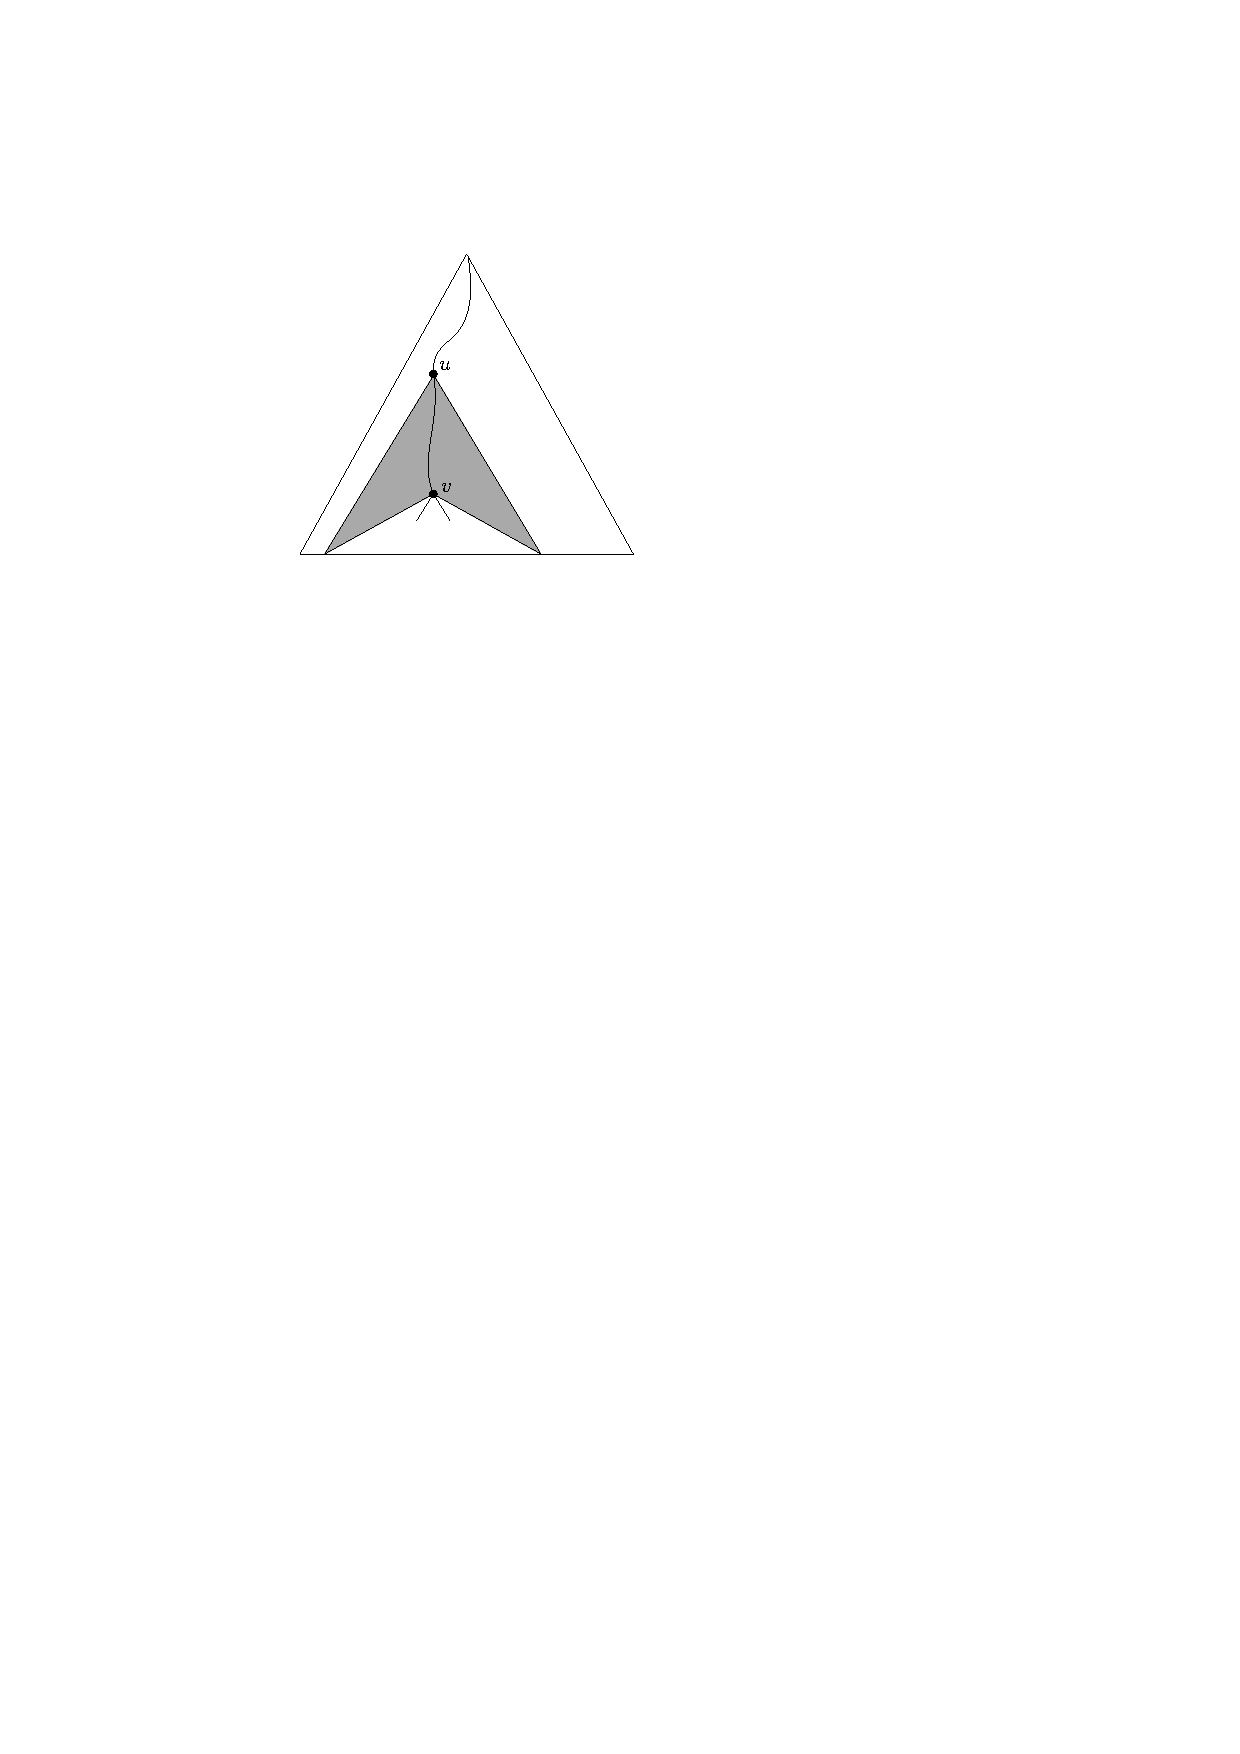
\includegraphics[scale=0.7]{fragment}
\end{center}
\caption{Example of a fragment in a good partition. The fragment consists of the subtree of $u$ without the subtree of $v$. We call $u$ the \emph{root} of the fragment and $v$ the \emph{hole} of the fragment. The path from $u$ to $v$ is called the \emph{spine} of the fragment.}
\end{figure}

\begin{lemma}\label{basic partitioning lemma}
For any binary tree on $n$ nodes and a parameter $b$, there is a good partition of the tree.
\end{lemma}
\begin{proof}
We prove the lemma by construction. Call a node \textit{large} if the size of its subtree is greater than $b$ and \textit{small} otherwise. Consider the tree $T_L$ induced by the large nodes of the original tree. Make each leaf in $T_L$ a new fragment with no hole. This creates $O(n/b)$ fragments since each leaf of $T_L$ is the root of a subtree of size at least $b$ in the original tree, and so we have at most $O(n/b)$ leaves in $T_L$. The size of each of these fragments is at most $2b$, since we assume that the tree is binary. Next, for every branching node in $T_L$, make it a fragment consisting of just one node. This also creates $O(n/b)$ fragments, since in any tree the number of branching nodes is at most the number of leaves. Notice that naively going up the tree and cutting fragments of size $b$, would not have worked, since this would create fragments with more than two boundary nodes. Ignoring the fragments we have already created, we are left with nodes that form unary chains in $T_L$. Each of these nodes might also have a child that is a small node. We have $O(n/b)$ of these subgraphs (because each of them is defined by two of the previously defined fragments). We scan each of these subgraphs' large nodes bottom-up, and greedily cut them into fragments of size at most $2b$. Denote the size of subgraph $i$, as $b_i$. The number of fragments we created in this phase is at most $$\sum_{i=1}^{n/b} \left\lceil \frac{b_i}{b} \right\rceil = O(n/b).$$
In total we have created $O(n/b)$ fragments, each of which is of size at most $2b$.
\end{proof}
This partitioning is done in $O(n)$ time.

\subsection{Pre-Processing fragments} \label{Pre-Processing Fragments}
We now would like to pre-process the fragments s.t. we can later check in constant time for any two nodes in a fragment, $u_1$ and $u_2$, if $d(u_1,u_2)\geq\lambda$, and if $d(u_1,u_2) \geq \frac{\lambda}{2}$, for any possible $\lambda$. The possible values of $\lambda$ in the beginning are of course all the pairwise distances in the input tree. We achieve the ability to perform such queries for most of the fragments, by using a parametric search method by Frederickson that allows us to eliminate some of the possible values of $\lambda$, using our existing feasibility test. By the end of this elimination process, most of the fragments will have the property that any pairwise distance inside them is either smaller then the smallest possible value of $\lambda$ or
 greater or equal to the largest possible value of $\lambda$. The same will hold for $\frac{\lambda}{2}$.
For each fragment, we will implicitly construct matrices of total side length (number of rows and columns) $O(b \log b)$, that are row and column sorted, and contain all pairwise distances in the fragment.

\begin{definition} \textbf{Centroid Decomposition}
A node $v\in T$ is a centroid if every connected component of $T\setminus\{v\}$ consists of at most $|T|/2$
nodes. The centroid decomposition of $T$ is defined recursively by first choosing a centroid $v\in T$
and then recursing on every connected component of $T\setminus\{v\}$ called \emph{pieces}.
\end{definition}

\begin{figure}
\begin{center}
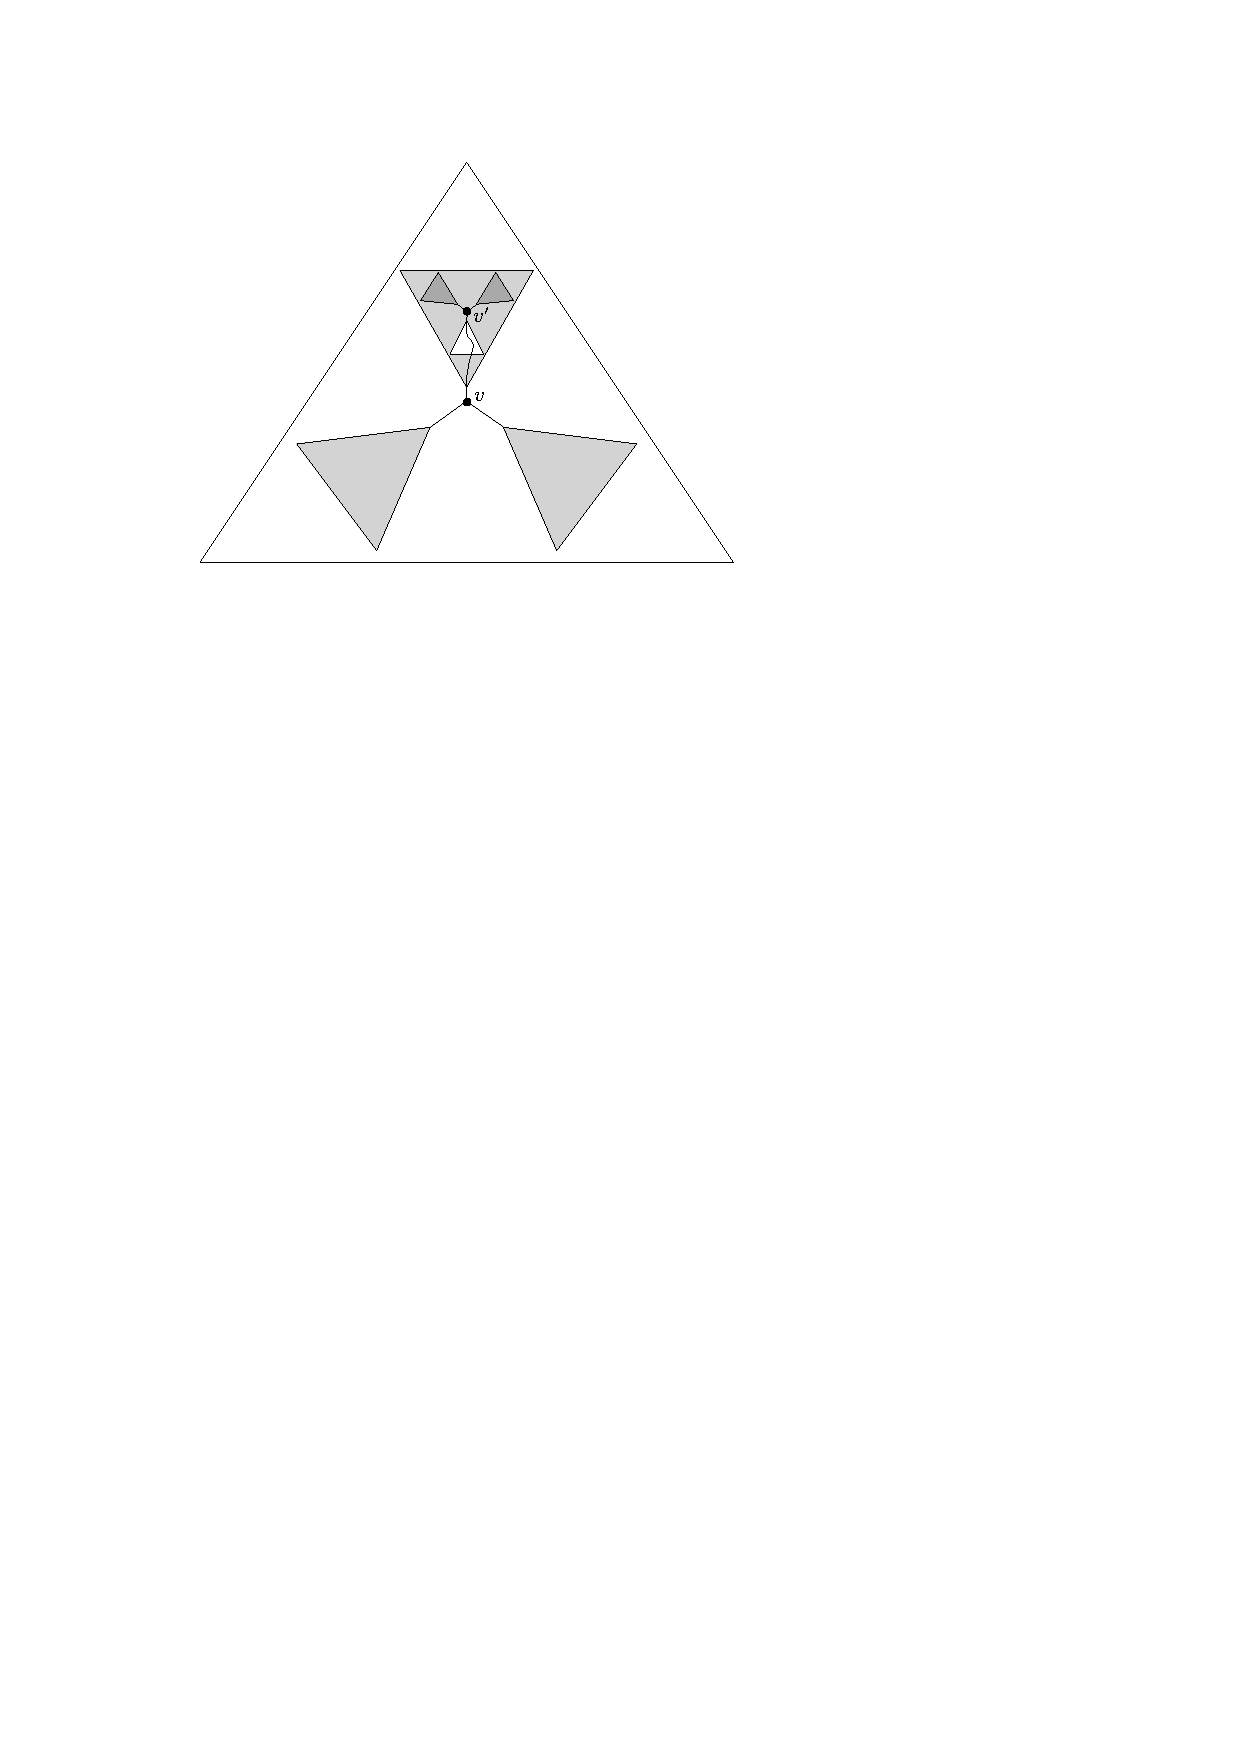
\includegraphics[scale=1]{centroid}
\end{center}
\caption{A single step in the centroid decomposition. Removing $v$ splits the tree into three pieces, s.t. none of them has more than $\frac{n}{2}$ nodes. The white piece is problematic, since the paths from its nodes to $v$ do not pass through the inner centroid $v'$.}
\end{figure}

Apply the centroid decomposition on each fragment. This take linear time. Since we assume our input tree is binary, the centroid at each level of the recursion will split the tree into three pieces. Now, run the following recursive routine: at each level of the recursion, we are given the three pieces of the decomposition, and for each of them a sorted list of the distances to their inner centroid. We would like to compute a sorted list of distances of the nodes in all three pieces, to the current centroid. This would give us the ability to compute, in constant time, the distance between any two nodes that are in different pieces (since the path between them goes through the centroid). Let us look at one of the three pieces we have already processed. It contains three pieces of its own. For two of these pieces, it holds that the path from every node inside them to the outer centroid passes through the inner centroid. We call the third piece, for which this does not hold a \textit{problematic} piece. For the two pieces that are not problematic, we can add to all the entries of the lists we have, the distance from the inner centroid to the outer centroid, and then merge the two sorted lists. This is all done in linear time.

Our only problem now is the piece where the paths to the outer centroid do not go through the inner one. But notice that if we go one step deeper in the recursion we can see that inside the problematic piece there are two pieces that are not problematic, as the paths from all their nodes to the outer centroid pass through their inner centroid. We can do the same kind of merging for their two list, and then look deeper inside the remaining problematic piece, and so on. This recursive routine will also take linear time. Altogether we have $O(\log b)$ levels of recursion, and spend linear time on each one, so we get a running time of $O(b \log b)$ per fragment. For now, we set $b$ to $\log ^2 n$ and get a running time of $O(\frac{n}{b} \times b\log b) = O(n \log \log n)$ for all fragments together.

Now we have for level $i$ of the recursion $3^i$ centroids, and for each of them a sorted list of the distances to all nodes in the appropriate pieces. We can find any pairwise distance in a piece by adding two entries of this list. Since the lists are sorted, we can look at the situation as if we have $3^i$ matrices of and their total side length is $n$ \footnote{We cannot actually afford to explicitly store these matrices, but that is not needed.}. The matrices from all levels of the recursion, contain all the pairwise distances inside all the fragments. Note that we also have some entries in the matrices that do not actually represent pairwise distances in the tree, because some entries in the matrix represent the length of a path between two nodes that passes through the centroid of the piece, but the shortest path between these two nodes does not pass through the centroid. This does not matter, since it just means we will do some unnecessary eliminations.

Now, we can use a parametric search algorithm by Frederickson to eliminate entries of the matrices. The idea of this method is looking at specific locations in the matrices, running feasibility tests on their values, and eliminating large pieces of the matrices. This is possible because these matrices are both row and column sorted, and because if some number $x$ is not a feasible solution for the dispersion problem, then any number $y>x$ is also not feasible, and also, if $x$ is feasible, then any number $z<x$ is also feasible. Using this searching method, we find the interval of possible solutions to the dispersion optimization problem \footnote{The possible solutions to the dispersion optimization problem are all the pairwise distances in the input tree. All of these distances are represented in entries of the matrices we have implicitly constructed.}, $[\lambda_1,\lambda_2)$, s.t. the $\lambda^*$ we are searching for is in this interval, $\lambda_1$ is the largest number we know is feasible, and $\lambda_2$ is the smallest number we know is not feasible. We call fragments that do not contain a pairwise distance that is in the interval \textit{inactive}, and all other fragments \textit{active}. Since we would like to also answer queries for $\frac{\lambda}{2}$, we do the same process for matrices that contain twice the distance in every entry of the original matrices.

For this search, we use Theorem 2.1 in \cite{Frederickson1991}:
\begin{theorem}\label{Frederickson's theorem}
Let $M$ be a collection of $N$ sorted matrices ${M_l, M_2, . . . , M_N}$ in which matrix $M_j$ is of dimension $m_j \times n_j$, $m_j \leq n_j$, and $\sum_{j=1}^{N} m_j = m$.
Let p be nonnegative. The number of feasibility tests needed to discard all but at most p of the elements is $O(\max \lbrace \log(\max_{j} \lbrace n_j \rbrace), \log(\frac{m}{p+1}) \rbrace)$, and the total running time exclusive of feasibility tests is $O(\sum_{j=1}^{N} m_j \times \log (2n_j/m_j))$.
\end{theorem}
In our case $m=b \log b \times \frac{n}{b} = n \log b$ (since for each of the $\frac{n}{b}$ fragments, we have $\log b$ levels of the centroid decomposition, and at each level we have the distance of every node to a centroid) and we set $p$ to be $n/b^2$. The theorem implies that we can use $O(\log b)$ feasibility tests and discard all but $n/b^2$ elements of the matrices. We also pay $O(n \log b)$ exclusive of the feasibility tests. This means that we have at most $n/b^2$ active fragments (out of all $n/b$ fragments). 

For inactive fragment, it is clear that we can now answer queries checking whether some pairwise distance inside the fragment is at least $\lambda$, or if it is less than $\frac{\lambda}{2}$ \footnote{We can easily compute any pairwise distance in the tree in $O(1)$ time by pre-computing all distances to the root of the tree, and using LCA queries \cite{Bender2000}, \cite{Djidjev1991}.}.

Active fragments will be processed as in the linear algorithm described before, so we can ignore them for now. We refer to the certain node which is closest to the root simply as \textit{the certain node}. We now do the following pre-processing for each inactive fragment:
\begin{enumerate}
\item\textbf{Reduce the fragment to a caterpillar:}\\
Observe that each fragment is comprised of its spine, and the subtrees hanging off of it. Using queries on pairwise distances as described above, we can use our linear feasibility test on the subtrees hanging off the spine, and get a candidate and a certain node for each of them. This is done in linear time.
Our fragment is now reduced to a caterpillar with at most two children for each spine node, a candidate child and a certain child.
\item\label{removing certain nodes}
\textbf{Find the candidate nodes that will certainly not be taken:}\\ %TODO add drawing
Let the $i$-th leaf of the caterpillar be connected by an edge of length $y_i$ to a spine node at distance $x_i$ from the root of the caterpillar. Order the leaves so that $x_1 < x_2 < ... < x_k$.
Some of the candidate nodes can be ignored as they "collide" with certain nodes. We start by finding the closest certain node to each candidate node. We can do this in linear time by scanning the caterpillar bottom-up, while saving for each candidate node, the closest certain node below it and the distance to it. We then do the same scan from top to bottom, and from both scans combined, we get for each candidate node the closest certain node and the distance to it. Now we want to find the candidate nodes that are too close to a certain node. We can do this since we are looking at an inactive fragment, and so a pairwise distance in it must be either smaller than $\lambda_1$ or greater or equal to $\lambda_2$. Delete all candidate nodes for which the distance to the closest certain node is smaller than $\lambda_1$. 
Now we are only left with some of the candidate nodes to consider, and for all of them it hold that $y_i < \lambda_1/2$ (otherwise they would be certain), and from this point we can ignore the certain nodes.
\item\label{making distances from the root monotone}
\textbf{Prune the caterpillar so that the leaves' distances to the root are non-decreasing:}\\
Traverse the caterpillar from bottom to top. Consider the $i$-th leaf, $u_i$, and the adjacent leaf above it, $u_{i-1}$. Assume $x_{i-1}+y_{i-1} > x_i+y_i$ (i.e. $u_{i-1}$ is farther from the root than $u_i$). We get that $x_i-x_{i-1}+y_i < y_{i-1}$. $d(u_i,u_{i-1}) = x_i-x_{i-1}+y_i+y_{i-1} < 2y_{i-1} < \lambda_1$. So an optimal solution cannot contain both $u_{i}$ and $u_{i-1}$. If $u_{i}$ is in the solution we can replace it with $u_{i-1}$. This can be done because $u_{i-1}$ is farther away from any node above it than $u_i$, and $u_i$ is closer to any node below it than $u_{i-1}$. Let $u_j$ be a leaf node above $u_{i-1}$ ($j<i-1$), then $d(u_j,u_{i-1}) - d(u_j,u_{i}) = y_{i-1}-(x_i-x_{i-1})-y_i = x_{i-1}+y_{i-1}-(x_i+y_i) > 0$. The reasoning for the second case (where $u_j$ is a leaf below $u_i$, i.e. $j>i$) is similar. So in fact, we can remove the $i$-th leaf from the caterpillar. We continue down the caterpillar in the same manner and remove leaves, until the distances of the leaves from the root non-decreasing.

\begin{figure}
\begin{center}
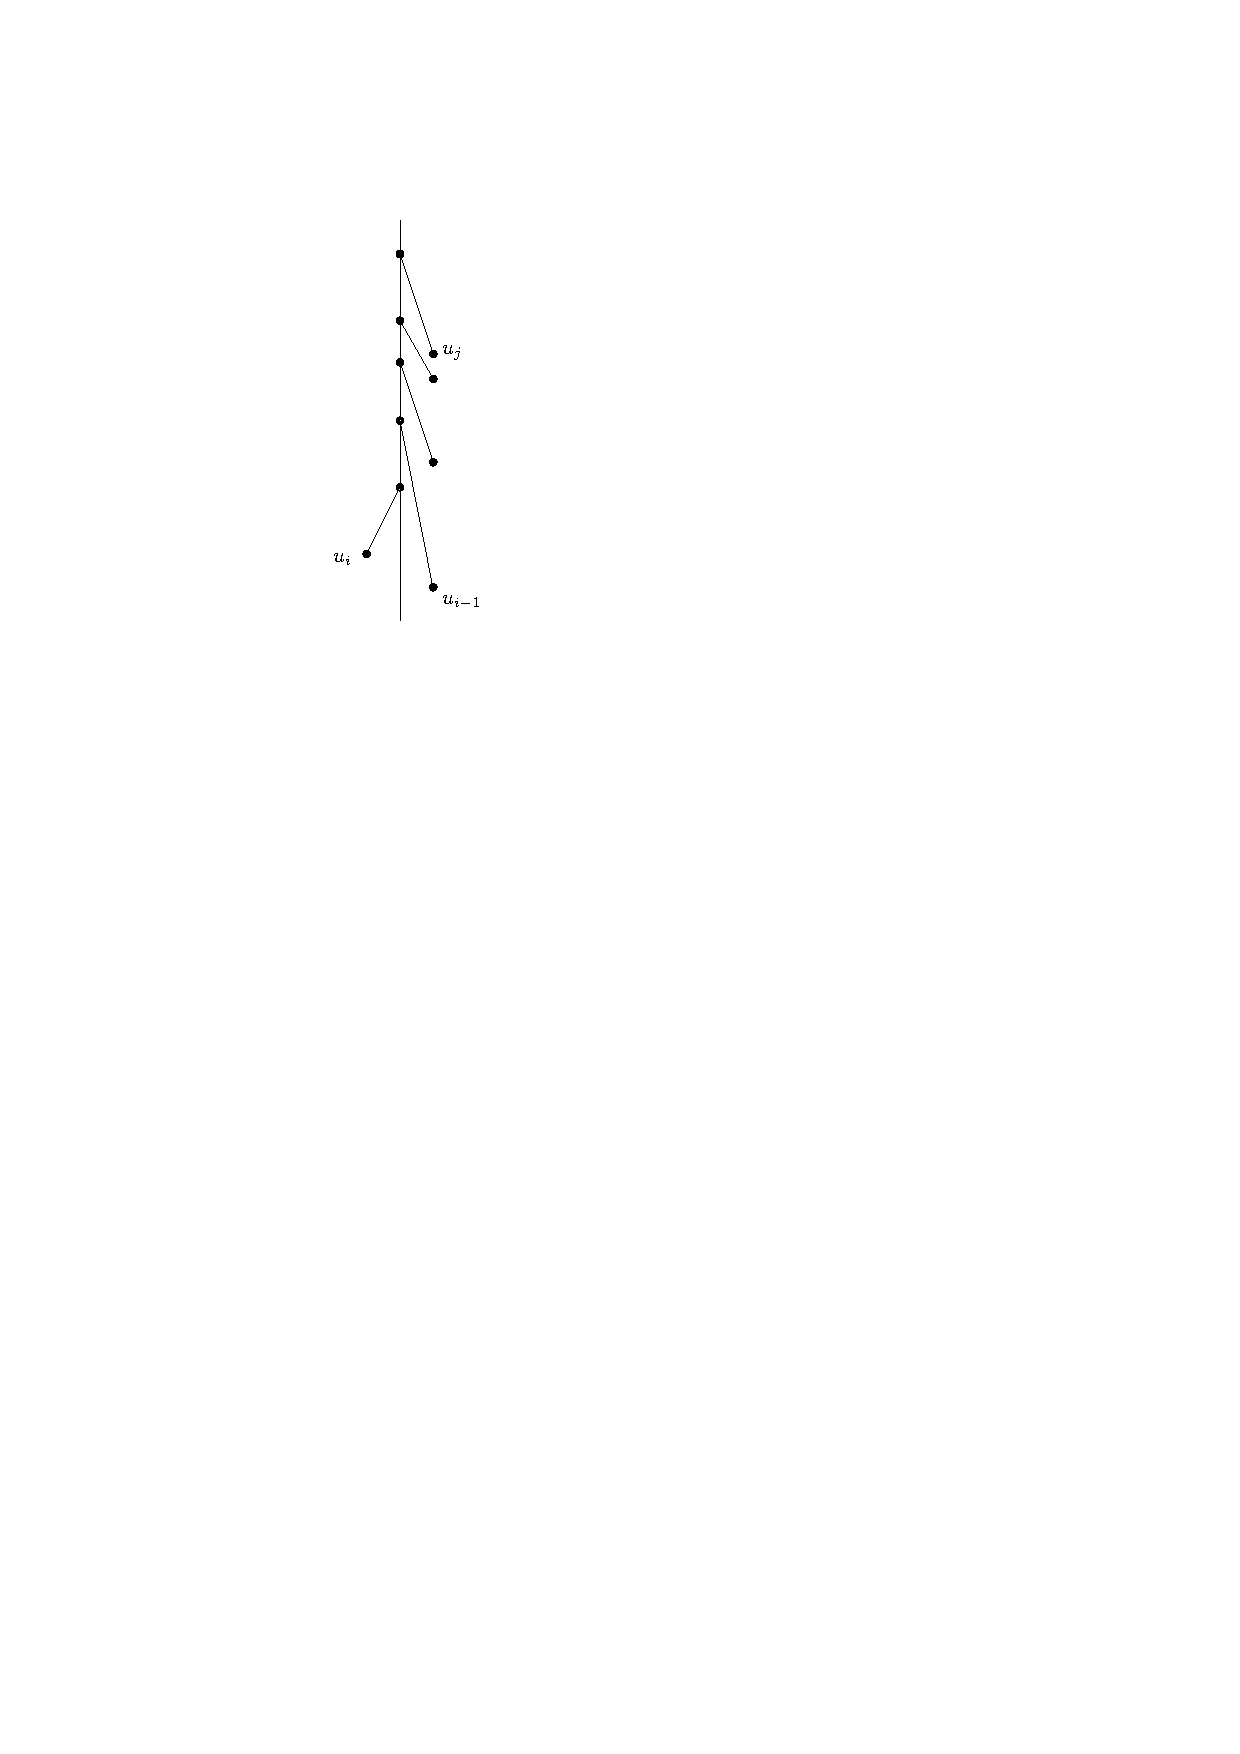
\includegraphics[scale=1]{caterpillar}
\end{center}
\caption{Pruning the caterpillar so that the distances of leaves from the root are non-decreasing. $d(u_i,r)<d(u_{i-1},r)$ and so we remove $u_{i}$. We can do this because any node from from above or below (e.g. $u_j$) is farther from $u_{i-1}$ than from $u_i$.}
\end{figure}

\item \label{making distances from the hole monotone}
\textbf{Prune the caterpillar so that the leaves' distances to the bottom are non-decreasing:}\\
This is done as in the previous step.
\item\textbf{Compute the solution for any possible distance of the hole's candidate node:}\\
In query time we want to process each fragment after its hole has already been processed.
We call a set of consecutive leaves of the caterpillar, that contains the closest leaf to the hole, a \emph{suffix} of the caterpillar. Similarly we can define the caterpillar's \emph{prefix}.
Assuming we know what is the closest chosen node in the fragment's hole, we can eliminate an entire suffix of the caterpillar (because of the monotonicity of the distances of candidate nodes from the hole). We can compute in preprocessing, for any possible eliminated suffix, which nodes in the fragment should be chosen, and also which nodes are the candidate and certain node we need to pass to the next fragment.
In order to pre-compute this, scan the caterpillar from top to bottom. For every possible prefix of the caterpillar we would like to store the numbers of nodes chosen, the certain node and the candidate node, assuming all nodes that are not in the prefix are eliminated as they are too close to the hole. Consider the bottom node of the current prefix. If the distance of this node to the fragment's root is less than $\frac{\lambda}{2}$\footnote{We do not actually know $\lambda$ in preprocessing, but due to the previous steps, such a query of a node inside the fragment would produce the same result for any possible $\lambda$.}, store it as the candidate node, zero as the number of chosen nodes, and NULL as the certain node (if this fragment has a hole, we will consider its candidate and certain node in query time). Else, (the node's distance to the root is greater or equal to $\frac{\lambda}{2}$), write it as the certain node. Then, use binary search to find the closest node above it, that is at distance of at least $\lambda$. Add 1 to the number of chosen nodes stored in the node we found, and either store it as the candidate node, or copy the candidate node stored there. This would take $O(b \log b)$ time. We can improve this by not binary searching for the first node far enough, but instead saving it for each prefix, and then only going down from the previous node found. This would only take $O(b)$ time.
\end{enumerate}

\subsection{Feasibility test}
We now scan the whole tree, and for each inactive fragment we would like to produce in $O(\log b)$ time: the number of chosen nodes in the fragment, the candidate node, and the certain node. In this procedure we use the caterpillars we have created in the preprocessing. We run this procedure bottom-up, so we assume that the fragment rooted at the hole of the current one has already been processed. Notice that now we are given $\lambda$. Denote the root of the fragment by $r$, and the current fragment's leaf which is farthest from $r$, by $v$.

If the hole does not have a candidate node, denote its certain node by $u$. We compute the suffix of the fragment that cannot be taken. We can do this by binary searching for the first node of the fragment that is at distance at least $\lambda$ (which is given now) from $u$. We have pre-computed all we need to know once we have the relevant prefix (i.e. the nodes we choose in the current fragment, including the certain and candidate nodes).

If the hole does have a candidate node, denote it by $u$. Assume $d(u,v) \geq \lambda$, then $u$ does not eliminate any suffix of the current fragment (due to the monotonicity of distances from the hole). Thus, we can take the nodes chosen so far, including the hole's candidate, $u$, and add to them the nodes we stored in preprocessing for the case that no suffix is eliminated. If $u$ and $v$ "collide" (i.e. $d(u,v) < \lambda$), we have the following two cases:
\begin{enumerate}
\item $d(r,v) > d(r,u)$: In this case, $v$ is farther from the root than $u$, which is possible since the monotonicity only holds inside each fragment. In this case we do not take $u$ into the solution, and only take the certain nodes we have so far. Because any certain node does not "collide" with $u$, it is also far enough from $v$, and so no suffix is eliminated and we take the appropriate nodes from the current fragment.
\item $d(r,v) \leq d(r,u)$: In this case we need to consider the suffixes of the current fragment, as in the case where the hole does not have a candidate.
\end{enumerate}
Each feasibility test costs us $O(\log b)$ for each inactive fragment, and $O(b)$ for each active one. In total $O(\frac{n}{b} \times \log b) + O(\frac{n}{b^2} \times b) = O(\frac{n \log \log n}{\log ^2n})$.


\section{$O(n\log\log n)$ Solution for the dispersion problem} \label{nloglogn solution}
The general idea of the algorithm is to use the heavy path decomposition. We are searching for $\lambda^*$, which is the distance between some two nodes in the tree, and the largest number for which a feasibility test would return true.
\begin{definition}
\emph{Heavy Path Decomposition} \cite{Sleator1983} Given a rooted tree, define the \emph{heavy edge} of each non-leaf node of the tree as the edge to the child that has the greatest number of descendants. These heavy edges form a decomposition of the tree into heavy paths. The heavy path decomposition induces a \emph{heavy path tree}, where each node corresponds to a path of the heavy path decomposition. For a path $p$ of the heavy path decomposition, $p$'s parent in the heavy path tree is the path that contains the parent of $p$'s topmost node. The heavy path tree has depth of at most $\log n$. %TODO what is a level?
\end{definition}
We go through the heavy path tree bottom-up, and process all heavy paths at a specific level in parallel, until we are left with a certain and candidate node for each of them. We maintain an interval $[\lambda_1,\lambda_2)$ as previously. The interval will get smaller and smaller throughout the run.

We now describe the processing of a heavy path, which is very similar to the preprocessing of inactive fragments presented in Subsection \ref{Pre-Processing Fragments}. Notice that the traversal is bottom-up, so we have already processed all of the path's children in the heavy path tree. Because we have determined $\lambda^*$ with sufficient accuracy (i.e. reduced the size of the maintained interval), each subtree hanging off a heavy path can be replaced by its candidate and certain node attached by single edges to the heavy path. Hence, each such heavy path is a caterpillar, with one or two children for each spine node. We would like to be able to find the certain and candidate nodes for the current heavy path. %The situation is illustrated in figure %TODO add a figure
Assume that the caterpillar has $k$ nodes. As we have defined before, let the $i$-th leaf be connected by an edge of length $y_i$ to a spine node at distance $x_i$ from the root of the caterpillar. Notice that $x_1 < x_2 < ... < x_k$.
\begin{enumerate}
\item\textbf{Find the candidate nodes that will certainly not be taken:}

This is done as in step \ref{removing certain nodes} in Subsection \ref{Pre-Processing Fragments}.
\item\textbf{Prune the caterpillar so that the distances of leaves from the root and the hole are monotone:}	

This is done as in steps \ref{making distances from the root monotone} and \ref{making distances from the hole monotone} in Subsection \ref{Pre-Processing Fragments}.
\item\textbf{Construct a row and column sorted matrix storing all pairwise distances in the caterpillar:}

We have obtained a caterpillar with one child for every spine node, s.t the distances of leaves are monotone. It is easy to see that arranging the matrix in the natural order will produce a triangular matrix with monotone rows and columns \footnote{Again, we cannot afford to explicitly store this matrix, but we can compute any pairwise distance in $O(1)$ time.}.
\item\textbf{Run a searching algorithm on the sorted matrices of all the heavy paths at the current level:}

We now use Theorem \ref{Frederickson's theorem} to search the sorted matrices containing all pairwise distances in the heavy paths of the current level. We need to eliminate all of the entries, and so we set $p$ to zero. We thus narrow down our interval $[\lambda_1,\lambda_2)$ so that it does not contain any pairwise distance in the caterpillar. Now, we can use the same bottom up procedure we used for the linear feasibility test in Section \ref{linear F.T.}, and produce a candidate and a certain node of the caterpillar that will be valid for any value of $\lambda^*$.
\end{enumerate}
Since the number of vertices in the heavy paths of the current level is at most $n$, we need to use $O(\log n)$ feasibility tests for each level. There are at most $\log n$ levels in the heavy path tree, so we use $O(\log ^2n)$ calls to our sublinear feasibility test in total. This yields a time complexity of $O(n \log \log n)$ (the time needed for the search exclusive of the feasibility tests is linear).

After processing all heavy paths we finally have a maximal valid solution for the whole tree.
Notice that throughout our algorithm we process caterpillars, and do not consider taking spine nodes to our solution. 
This is fine, since we can attach to every such spine node an artificial leaf connected with an edge of length zero.
The same trick allows us to handle non-binary trees: given a non-binary tree, we can replace every 
degree $d\geq 3$ node with a binary tree on $d$ leaves. The edges of the binary tree are all of length zero and
its artificial inner nodes cannot be taken (notice that our algorithm easily generalises so that for each node
we can specify if it can be included in a solution).

\section{$O(n\log^{*}n)$ Algorithm}
The high level idea of the $O(n \log \log n)$ algorithm was dividing the input tree into fragments, and preprocessing them using the linear feasibility test (or test for short) to get a sublinear one. In order to get the complexity down to $O(n \log ^*n)$ we will use a similar process, iteratively, with growing fragments size, improving in each iteration the performance of our test.
We start with fragments of size $c^3$ for some constant $c$.
We pay $O(n)$ time for preprocessing and get an $O(\frac{n}{c^3} \times \log c)$ time test.
We use this test to do the same preprocessing again, this time with fragments of size $(2^c)^3$.
We will now achieve $O(\frac{n}{2^{3c}} \times c)$ time for test.
We do this for $\log ^*n$ iterations until we get to fragments of size $\log ^3n$, and have an $O(\frac{n \log \log n}{\log ^3n})$ time test. Since we do $\log ^*n$ iterations and linear time work for each of them the total preprocessing is in $O(n \log ^*n)$ time.

We now describe one iteration of this process. Assuming we have obtained an $O(\frac{n}{b^3} \times \log b)$ time test from the previous step, we now find a good partition of the tree, with fragments of size $B^3$, where $B:=2^b$. We perform a heavy path decomposition on each fragment, and go over the heavy path trees of the fragments bottom up and in parallel. The paths at lower levels have been processed s.t. each of them is reduced to a candidate and a certain node, and so each current path is a caterpillar, that we will now reduce to two nodes by using Frederickson's method. As we have seen in Section \ref{nloglogn solution}, we can create a matrix with linear number of rows and columns, that contains all pairwise distances of a path at the current level. We construct each matrix by pruning the caterpillars so that the distances of leaves from the root and the hole are monotone, thus achieving a matrix that is row and column sorted. For each level of the heavy path decomposition we have $O(n/B^3)$ matrices of size at most $n$ for all fragments together (since each heavy path contains at most all the vertices of the fragment). We use Frederickson's searching method, with the parameters $m=n$ and $p:=\frac{n}{B^4}$. We thus need to use the test $O(\log (\frac{n}{\frac{n}{B^4}}))=O(\log B)$ times, and an extra linear processing time exclusive of the feasibility tests. We compute the candidate and certain node of each path as we did before, and continue up in the heavy path trees, until we are left with only the top heavy path of each fragment. Since $p>0$, during this preprocessing, some fragments become active. Once a fragment becomes active we stop its preprocessing.

After the preprocessing is done, we have at most $\log B \times \frac{n}{B^4}$ active fragments (because we do not eliminate at most $p$ pairwise distances at each level), which we will process in linear time in the new test. For all other fragments we have obtained a pruned caterpillar, so that we can, in linear time, pre-compute the required information for any possible eliminated suffix as described in Subsection \ref{Pre-Processing Fragments}. We will process these inactive fragments in logarithmic time in the new test Thus we have obtained a test of $O(\frac{n}{B^3} \times \log B)$.

We do this iteratively until we have an $O(\frac{n}{\log ^3n} \times \log \log n)$ time test, and then use it solve the dispersion optimization problem in linear time (in the same manner as in each of the previous $\log ^*n$ iterations, this time with only one fragment of size $n$). In total, for all $O(\log B)$ levels of the heavy path trees, we used $O(\log ^2B)$ calls to the previous test, that cost $(\log ^2B \times \frac{n}{b^3} \times \log b)=O(\frac{n}{b} \times \log b)$ which is less than linear time. In addition, at each step we used linear time for the decompositions, so in total $O(n \log ^*n)$. 

\section{Linear time solution for the dispersion optimization problem}
Our linear algorithm is based on the $O(n \log ^*n)$ algorithm we have presented. In order to achieve linear time in total we cannot partition the input tree to fragments independently for each fragment size. We need the decomposition into fragments to take $O(n)$ time for all $\log ^*n$ iterations together.
\begin{lemma}\label{good partition refinement lemma}
Given a good partition of a binary tree into $O(n/b)$ fragments s.t. each fragment is of size at most $2b$, there exists a good partition of the tree into $O(n/2^b)$ such fragments of size at most $2 \times 2^b$, so that every small fragment is contained inside a large fragment.
\end{lemma}
\begin{proof}
Define $T'$ by the tree received by collapsing each small fragment (of the given partition) to a single node. Apply Lemma \ref{basic partitioning lemma} to $T'$, with the parameter set to $B:= \frac{2^{b-1}}{b}$. We get $O(\frac{\frac{n}{b}}{B})=O(\frac{n}{2^b})$ fragments, each of which of size at most $2 \times B \times 2b = 2 \times 2^b$.
\end{proof}
We now describe a single iteration, i.e. how to construct an $O(\frac{n}{B^4} \times \log B)$ time test, given an $O(\frac{n}{b^4} \times \log b)$ test and a good partition of the input tree into fragments of size $b^4$. We start by applying Lemma \ref{good partition refinement lemma}, and constructing a good partition with $O(\frac{n}{B^4})$ fragments of size $O(B^4)$. This takes $O(\frac{n}{b^4})$ time.

Consider a large fragment of size $B^4$. It contains some small fragments of size $b^4$. Notice that some of these are active fragments, that might be full subtrees (i.e. have not been reduced to caterpillars in previous levels), but almost all of them are inactive smaller fragments, which have been reduced to caterpillars. The large fragment contains some small fragments whose roots and holes are spine nodes of the large fragment, and other fragments that form subtrees hanging off of the large fragment's spine (each hanging subtree may contain several small fragments). See Figure \ref{figure of small fragments inside a large frament}.

\begin{figure}\label{figure of small fragments inside a large frament}
\begin{center}
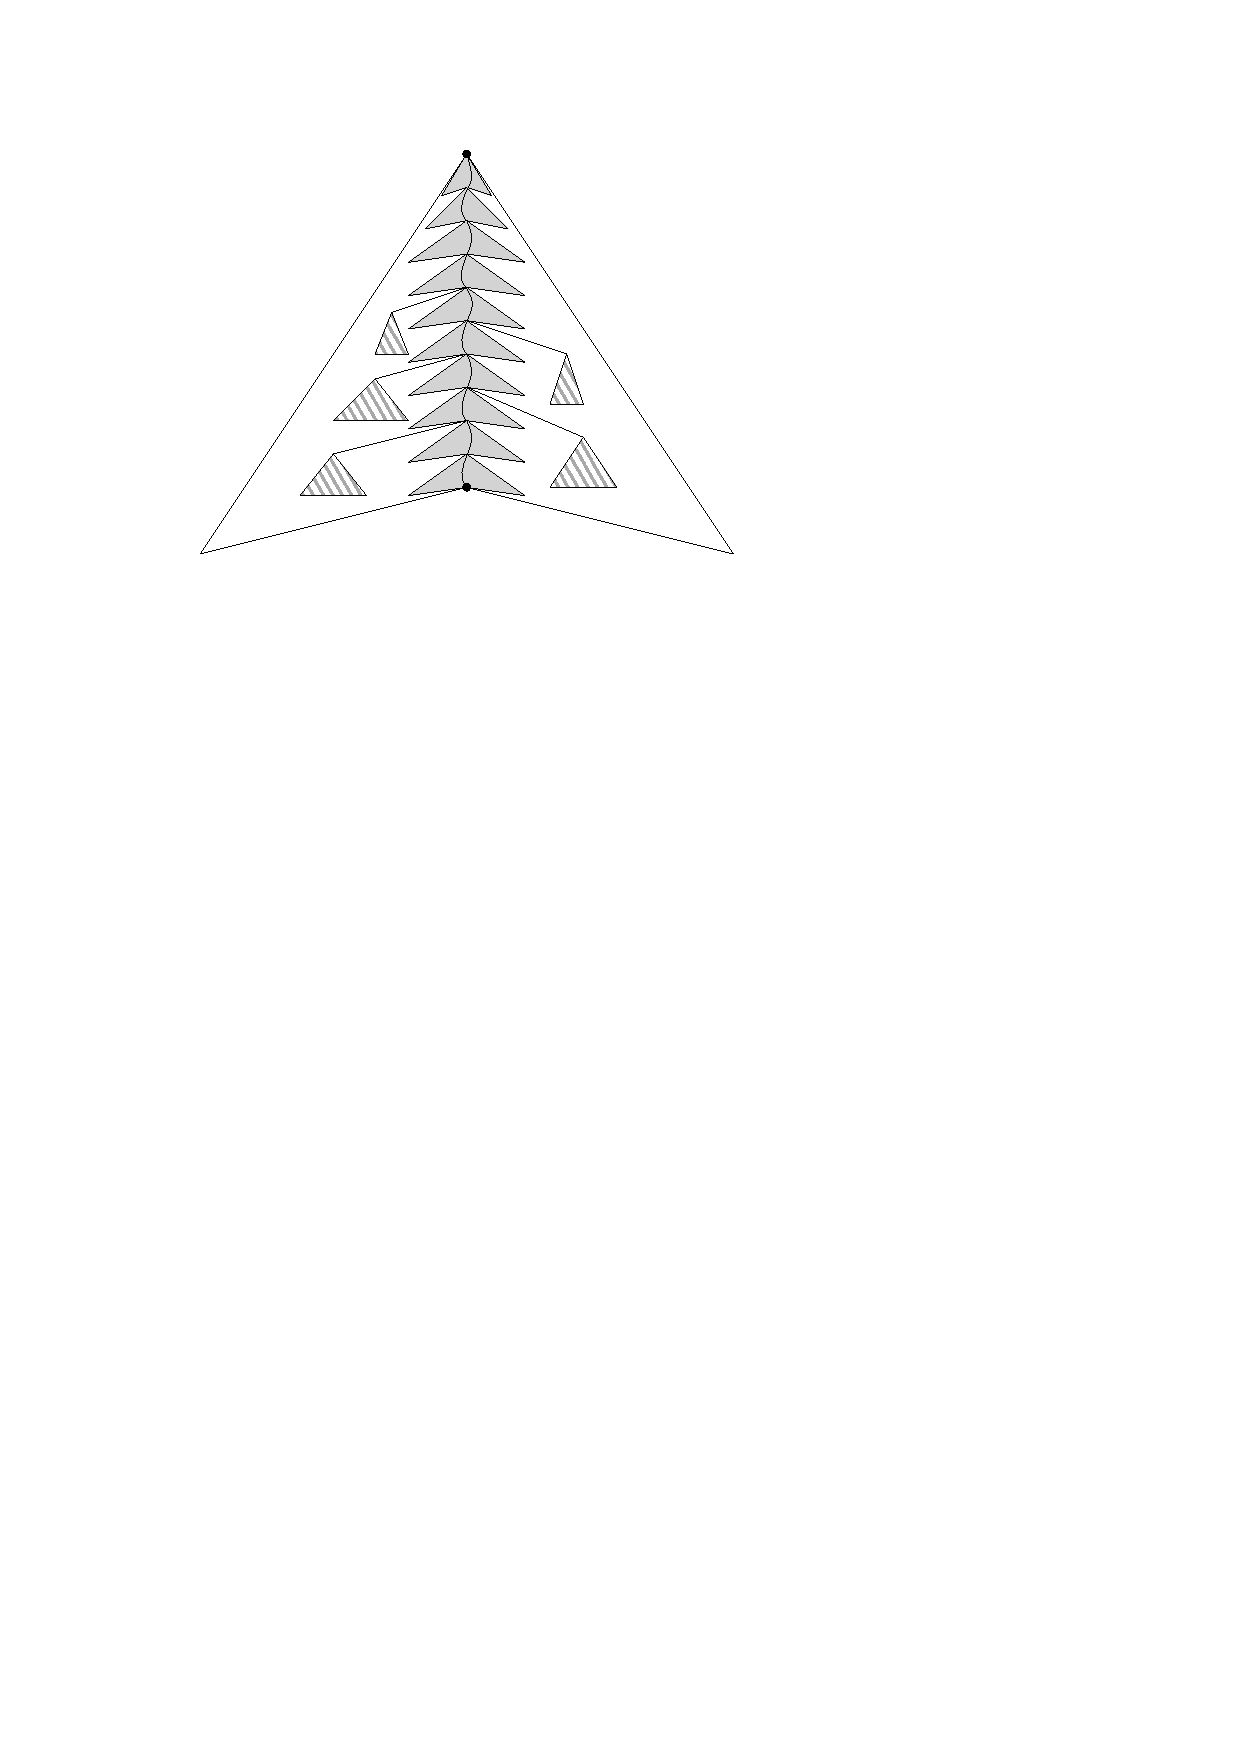
\includegraphics[scale=1]{refinement}
\end{center}
\caption{A large fragment containing a number of smaller fragments. The small fragments on the spine are in gray, and the subtrees hanging off of the spine are striped. We start by reducing the hanging subtrees to just two nodes, then handle the small active fragments on the spine, and finally reduce the entire large fragment to one caterpillar and process it.}
\end{figure}

We first reduce each of these hanging subtrees to at most two nodes, one candidate and one certain. To do this, we perform a heavy path decomposition on each of them. Since each subtree like this is contained in one large fragment, its size is bounded by $B^4$, and so we have at most $O(\log B)$ levels in the heavy path decompositions. On each level we run Frederickson's search (similarly to what we presented before). We run this search in parallel, for all the heavy paths from all these hanging subtrees in all the large fragments. The number of nodes in the current level for all the heavy path trees together is at most $n$. We set the parameter $p$ to $\frac{n}{B^5}$. Aside from linear (in the number of nodes in these subtrees) time processing exclusive of tests we need to call our $(\frac{n}{b^4} \times \log b)$ test $O(\log B)$ times for each of the $O(\log B)$ levels. This takes $O(\frac{n}{b^2} \times \log b) = O(\frac{n}{b})$. Denote the size of the small fragments at iteration $i$ by $b_i$ ($b_i=2^{b_{i-1}}$). For all $\log ^*n$ iterations of the algorithm the cost of these feasibility tests is bounded by $O(\sum_{i=0}^{\log^*n} \frac{n}{b_i}) = O(n)$.

Since each hanging subtree is contained inside a single large fragment, we can now reduce the subtrees to at most two nodes, one candidate and one certain node for each subtree. The heavy path decomposition we performed on the subtrees takes linear time, but each such subtree is reduced, and its nodes will not be processed in future iterations, and so this takes $O(n)$ time over all iterations. The exception to this is that we set the parameter $p$ of Frederickson's method to $\frac{n}{B^5}$, and thus there are at most $\frac{n}{B^5}$ large fragments in which we cannot reduce the hanging subtrees. These fragments become active fragments. The number of nodes in such fragments in a single iteration is at most $\frac{n}{B^5} \times O(B^4) = O(\frac{n}{B})$. The amortized style argument above does not hold for these vertices, since their subtrees are not reduced and they will be processed in future iterations, but we can afford to pay $O(\frac{n}{B})$ per iteration (as this sums up to $O(n)$ overall).

Notice that we do not mind if some of the small fragments in the hanging subtree had been active, but we now have to to deal with active small fragments that are on the spine of the large fragment. In the previous level we had $O(\frac{n}{b^5})$ active fragments, which is of course too many for the current level. We take the remaining active small fragments (which are on the spines of large fragments), and reduce them to caterpillars. We do this as in the $O(n \log^* n)$ algorithm. Each time we run the Frederickson method we set $p$ to $\frac{n}{B^5}$. In each fragment we have $O(\log b)$ levels of the heavy path decomposition, and for each level we need $O(\log B)$ calls to the feasibility test, which take  $O(\frac{n}{b^4} \times \log b \times \log B \times \log b) = O(\frac{n}{b})$ time in total. We also do linear work exclusive of feasibility tests. This processing of small active fragments takes $O(n)$ time over all $\log ^*n$ iterations, by the same reasoning as for the hanging subtrees.

We now have $O(\frac{n}{B^5})$ active small fragments in total. We declare each large fragment that contains a small active fragment as active. For each of the inactive large fragments, we are left with one large caterpillar which is the large fragment's spine, that consists of concatenated caterpillars from the smaller fragments. We want to process this caterpillar as we have processed inactive fragments before, and have a large caterpillar that has the necessary properties. The leaves' distances from the root and hole need to be monotone, and there should be no collisions between candidate nodes and certain nodes in the caterpillar. Once we have these properties, we will be able to preprocess the caterpillar for every possible eliminated suffix.

We start by pruning the large caterpillar so the candidate nodes' distances from the root and hole are monotone. Since the candidate nodes' distances are monotone inside each small caterpillar, we only have to check the last candidate node of a caterpillar against a consecutive subset of the candidates below it in the large caterpillar, starting from the closest node from below. We go over the large caterpillar from top to bottom, and for the last candidate of each small caterpillar we eliminate the appropriate candidates below   it. Now the distances of the candidates in the large fragment from the root are non-decreasing. We do the same process, this time from bottom to top, and check the first candidate node of each caterpillar against a continues set of leaves, starting from the closest leaf from above. Since we only had to check a continues part of the caterpillar each time, this step is done in time linear in the number of nodes eliminated, and $O(n)$ overall.

Now we need to eliminate all internal "collisions" inside the caterpillar (i.e. remove the candidate nodes that are too close to certain nodes). These collisions can occur between a candidate node of one small caterpillar, and a certain node of another small caterpillar. Each certain node eliminates candidate nodes that form a continuous part of the large caterpillar that is adjacent to the certain node's small caterpillar. Because of the monotonicity of distances of leaves inside each small caterpillar, we only need to consider the top-most and bottom-most certain nodes of each small caterpillar. We can create a matrix of dimension $1 \times B$ for each of these $O(\frac{n}{b^4})$ certain nodes (in the whole tree). Using Frederickson's method with $p$ set to $\frac{n}{B^5}$ costs us $O(\max \lbrace \log(\max_{j} \lbrace n_j \rbrace), \log(\frac{m}{p+1}) \rbrace) = O(\max \lbrace \log B, \log(\frac{\frac{n}{b^4}}{p} \rbrace) = O(\max \lbrace \log B, \log(\frac{B^5}{b^4} \rbrace) = O(\log B)$ calls to tests and $O(\frac{n}{b^4} \times \log B) = O(\frac{n}{b})$ for processing exclusive of feasibility tests.

The problem with eliminating collisions in this way, is that we assume that the implicit matrices on which we search, and contain the distances from a certain node to all candidates above it or below it, can be randomly accessed. As we have mentioned before, given two nodes in the input tree we can calculate the distance between them in constant time. But, in order to perform a feasibility test with some value in one of these $1 \times B$ matrices, say the value in the middle, we need to know which node we need to compute the distance to. This is similar to trying to binary search over a linked list. We cannot store these caterpillars in arrays, because they would not fit the processing we have been doing so far (e.g. pruning would be difficult with arrays). In the previous $O(n \log \log n)$ and $O(n \log ^*n)$ algorithms, we had no such problem, as we could go over the caterpillar in linear time and insert the candidates we want into an array. Now, we cannot afford linear time processing in each iteration. Fortunately, we do not have to preform such random accesses in $O(1)$, and $O(\log B)$ will suffice. For this, we store each caterpillar in a balanced search tree (BST). Merging the small trees of size $b$ to large trees of size $B$ takes $O(\frac{n}{b^4} \times \log B)$ time, since merging BSTs is done in logarithmic time. Since the access to our BST is done in logarithmic time, we need to multiply the complexity we have shown for this step of eliminating collision by $O(\log B)$, but this is still good enough.

We are now left with only the candidate nodes to consider, and we need to pre-compute for every possible eliminated suffix of every inactive large fragment, the number of chosen nodes in it and the candidate and certain nodes. In the previous algorithm, we stored at the bottom node of every prefix of the fragment, the number of chosen nodes, the candidate node and the certain node for this fragment, in case the suffix of the caterpillar below this node is eliminated. Now, we cannot afford to store all three fields for every node in every iteration of the algorithm (i.e. for each fragment size), as that would take linear time per iteration. We only store for each candidate in the caterpillar, a \emph{jump pointer} to the closest candidate above it that is at distance at least $\lambda ^*$ from it. Assuming the jump pointers inside every small caterpillar have already been computed, we would like to compute the jump pointers for the large caterpillar. We will do this iteratively, by merging pairs of small caterpillars each time. We start with merging pairs of small caterpillars, then merge pairs of the resulting caterpillars, and so on. 

Consider two consecutive caterpillars we want to merge. Each such caterpillar is of size $x$, where $2b \leq x \leq 2B$. Notice that for the upper caterpillar we only need to look at a suffix of it s.t. the highest node in the suffix is the lowest node in the upper caterpillar that is at distance greater or equal to $\lambda ^*$ from any node below it in the upper caterpillar (i.e. the lowest node that has a jump pointer pointing to it). Call this suffix the \emph{interesting suffix} of the upper caterpillar. Of course the jump pointer of any node in the lower caterpillar, cannot point to a node higher than this suffix. Similarly, we are only interested in a prefix of the lower caterpillar s.t. the lowest node in the prefix is the lowest node that does not have its jump pointer pointing to a node in the lower caterpillar. Call this prefix the \emph{interesting prefix} of the lower caterpillar. We now update these jump pointers. We go over the interesting prefix of the lower caterpillar bottom-up. For each node, first check if its distance to the highest node of the upper caterpillar's interesting suffix is greater or equal to $\lambda ^*$. If not, stop (this can only happen if the interesting suffix is actually the whole upper caterpillar). Else, go over the interesting suffix bottom-up, and find the first node that is at distance greater or equal to $\lambda ^*$ from the current node. Save the node found in the jump pointer, and for the next node in the interesting prefix we can start searching from this node. The problem here is that we do not have $\lambda^*$, and we can not check if a node in the lower caterpillar is at distance smaller than $\lambda^*$ from a node in the upper caterpillar or not. For that we need to run the Frederickson method once more. Since we have pruned the large caterpillar s.t. the distances of leaves from the root and hole are monotone, we can now run the search method on the nodes of the interesting prefix and suffix. We are only interested in distances between nodes of the interesting prefix to nodes in the interesting suffix, so we have a matrix for each node of the interesting prefix of dimension $1 \times x$ in the worst case (i.e. the distances from a single node in the interesting prefix  to all the nodes in the interesting suffix). We do this for all pairs of adjacent caterpillars, so we have at most $O(\frac{n}{x^4} \times x)$ such matrices. We set $p$ to $\frac{n}{B^5}$ again, and we need only $O(\log B)$ feasibility tests. The search also requires $O(\frac{n}{x^3} \times \log x)$ time for processing exclusive of feasibility tests. We can now answer the necessary queries for updating jump pointers.

%After we have updated jump pointers for every pair of adjacent small caterpillars, we join them, and make each such pair a new small caterpillar, and continue in the same manner, until we have updated all the jump pointers for every large caterpillar.
We do $O(\log B)$ such iterations until we have updated all the jump pointers for every large caterpillar. For updating jump pointers, we only spend time linear in the number of nodes whose jump pointer was updated. Every such node will not be in an interesting prefix again in future iterations. Thus we spend $O(n)$ time over all iterations. After the last iteration, we use the jump pointers to also update for each candidate node in all inactive fragments, the fields of certain and candidate node in case this is the first node above the eliminated suffix of the fragment. This can easily be done in $O(n)$ time. %TODO add drawing

Because we have set the parameter $p$ of Frederickson's method to at most $\frac{n}{B^5}$, this is the number of active fragments for the current iteration, in the worst case. Thus, we have achieved a $O(\frac{n}{B^4} \times \log B)$ feasibility test. After $\log ^*n$ iterations, we have a $O(\frac{n}{\log ^4n} \times \log \log n)$ test, which we use to solve the dispersion optimization problem in linear time. All iterations of pre-processing cost $O(n)$ time altogether.

\bibliographystyle{abbrv}
\bibliography{dispersion}



\end{document}